\chapter{The $\mathbf{\text{{\bf CL}}_s}$ Method}
\label{sec:cls}

In the absence of an excess compatible with a signal hypothesis, we define 95\% confidence level (CL) exclusion limits on model parameters such as cross sections and particle masses.
The method used here was first used for the combination of CMS and ATLAS results for the Higgs search~\cite{cls1} and is based on earlier approaches from many other particle physics experiments~\cite{cls2,cls3}.
Given an analysis-specific likelihood $\La$, we define the test statistic as:
\begin{equation}
    \tilde q_\mu^\mathrm{obs} = -2\ln \frac{\La(\bm{d}_\mathrm{obs} \,|\, \mu,\hat{\bm{\theta}}_\mu)}{\La(\bm{d}_\mathrm{obs} \,|\, \hat\mu,\hat{\bm{\theta}})}
\end{equation}
where $\bm{d}_\mathrm{obs}$ is a vector of observations in data; $\mu$ is a free parameter corresponding to the signal strength; and the nuisance parameter estimates are:
\begin{gather}
    \hat{\bm{\theta}}_\mu = \argmax_{\bm{\theta}} \La(\bm{d}_\mathrm{obs}\,|\,\mu,\bm{\theta}) \nonumber \\
    \hat\mu, \hat{\bm{\theta}}_\mu = \argmax_{\bm{\theta}} \La(\bm{d}_\mathrm{obs}\,|\,\mu,\bm{\theta}) 
\end{gather}
We further require that $0 \leq \hat\mu \leq \mu$, as the goal of $\tilde q _\mu$ is to measure the compatibility of the data with a non-negative signal strength smaller than the hypothesis $\mu$.

To estimate the significance of the measured $\tilde q^\mathrm{obs}_\mu$, we generate \emph{pseudo-data} by using the likelihood as a generative model.
The pseudo-data follows the distribution:
\begin{equation}
    \bm{d}_{\bar\mu} \sim \La(\bm d\,|\,\bar\mu, \hat{\bm{\theta}}_{\bar\mu})
\end{equation}
This leads to a natural definition of the conditional test statistic:
\begin{equation}
    \tilde q_{\mu}\,|\,{\bar\mu},\hat{\bm\theta}_{\bar\mu} = -2\ln \frac{\La(\bm{d}_{\bar\mu} \,|\, {\mu},\hat{\bm{\theta}}_{\mu})}{\La(\bm{d}_{\bar\mu} \,|\, \hat{\mu},\hat{\bm{\theta}})}
\end{equation}
With a sufficiently large pseudo-dataset $\{\bm{d}_{\bar\mu}\}$, we estimate the probability distribution function $p(\tilde q_{\mu}\,|\,{\bar\mu},\hat{\bm{\theta}}_{\bar\mu})$.
Finally, we define the $\CLs$~statistic as:
\begin{gather}
    \CLs(\mu) = \frac{\mathrm{CL}_{s+b}(\mu)}{\mathrm{CL}_b(\mu)},~\text{where:} \nonumber \\ 
    \mathrm{CL}_{s+b}(\mu) = \int_{\tilde q_\mu^\mathrm{obs}}^\infty \di \tilde q_{\mu}~p(\tilde q_\mu\,|\,\mu,\hat{\bm{\theta}}_\mu), \quad
    \mathrm{CL}_b(\mu) = \int_{\tilde q_\mu^\mathrm{obs}}^\infty \di \tilde q_{\mu}~p(\tilde q_\mu\,|\,0,\hat{\bm{\theta}}_0)
\end{gather}
These PDFs and the corresponding integrals are shown in Figure~\ref{fig:cls:cls}.

\begin{figure}[]
    \begin{center}
        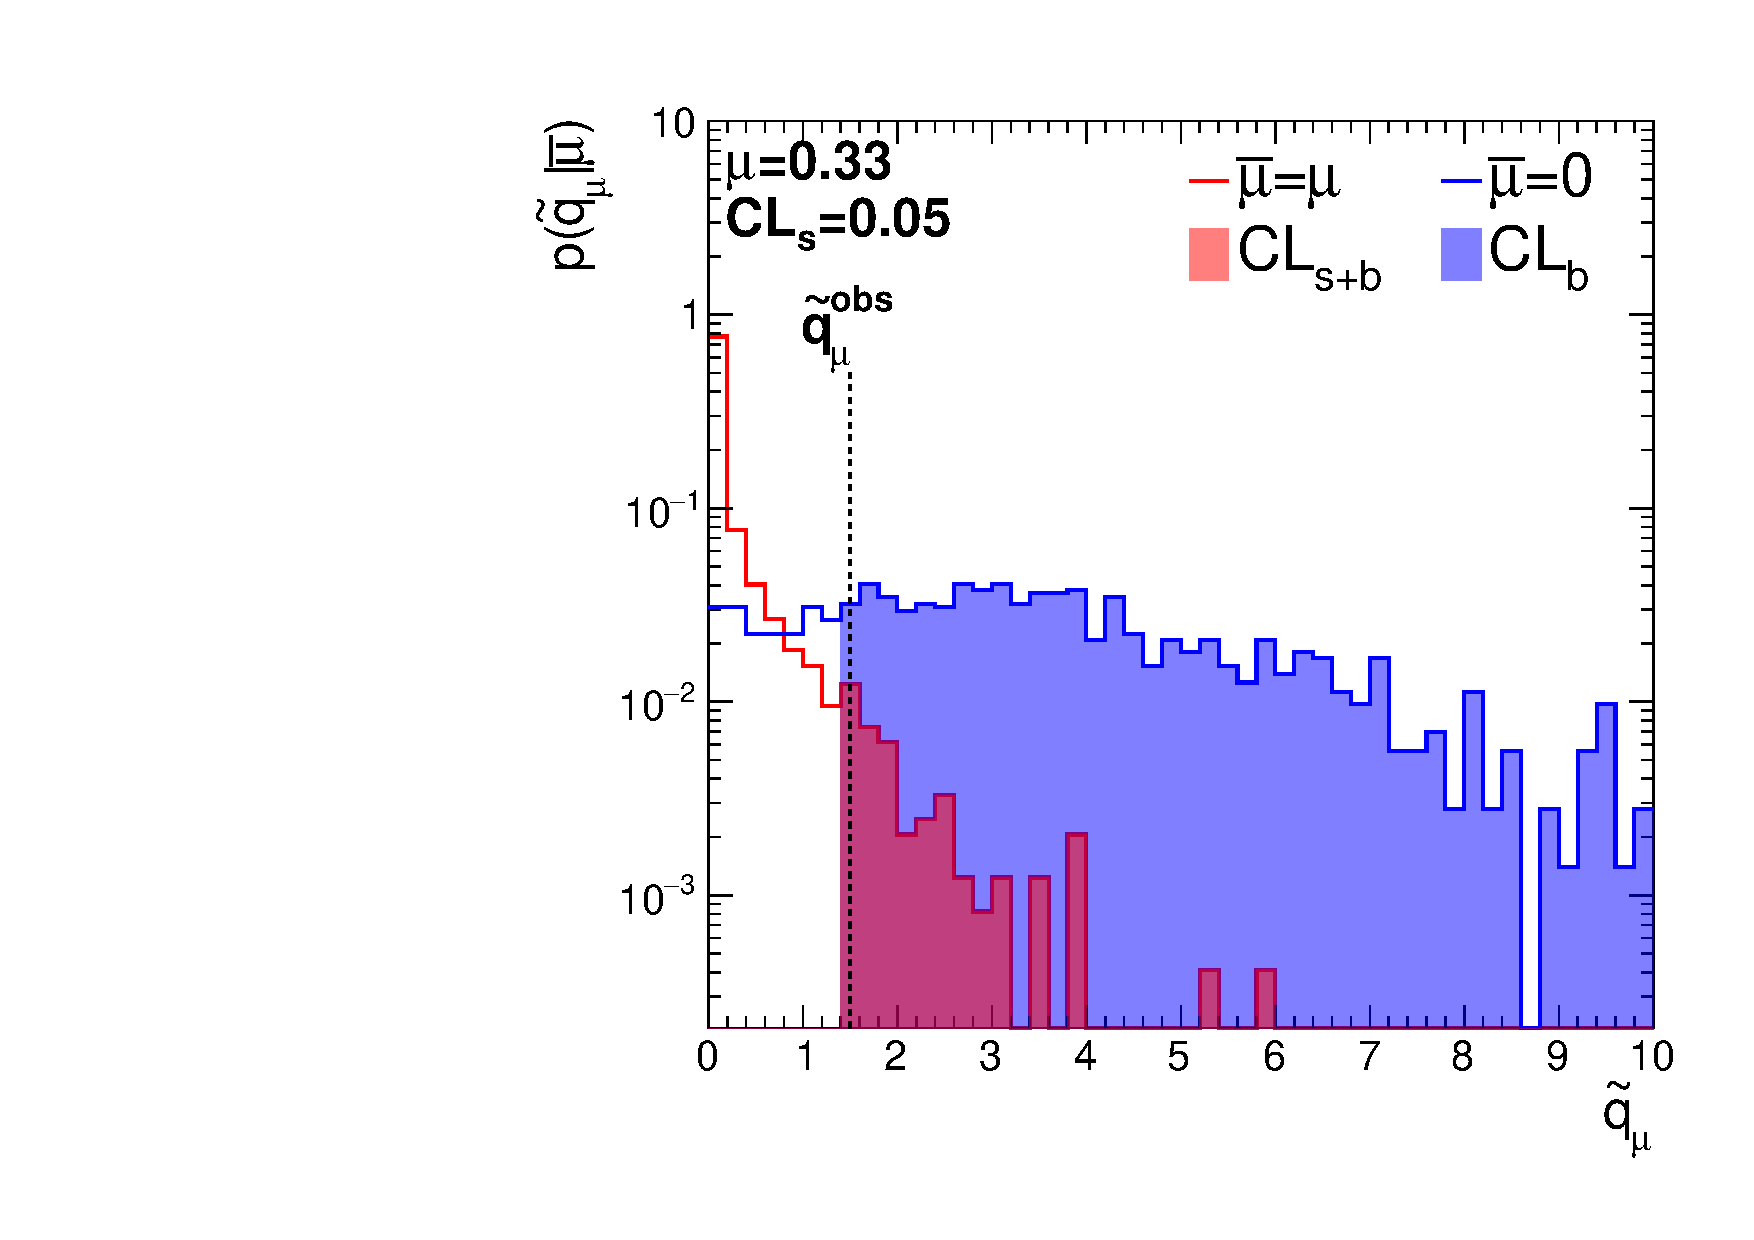
\includegraphics[width=0.5\textwidth]{figures/cls/cls.pdf}
        \caption{Distribution of $p(\tilde q_\mu\,|\,\mu)$ and $p(\tilde q_\mu\,|\,0)$ at $\mu = 0.33$. 
                 This value is chosen because it gives $\CLs(\mu) = 0.05$, corresponding to the $95\%$ upper limit.
                 The likelihood in this case is the VBF \hinv~analysis discussed in Chapter~\ref{sec:vbf}.}
        \label{fig:cls:cls}
    \end{center}
\end{figure}

If $\CLs(\mu) = 1-\alpha$, then we say the signal with strength $\mu$ has been excluded at $\alpha$ confidence level ($\mu_\alpha^\mathrm{obs}$).
One can also identify $\CLsb$ as a $p$-value, but it does not take into account the sensitivity of the data to the differences between the background-only and signal+background models.
By construction, $\CLb \leq 1$, which acts as a penalty as $p(\tilde q_\mu | 0)$ approaches $p(\tilde q_\mu | \mu)$.

To estimate the significance of $\mu_\alpha^\mathrm{obs}$, the above procedure is repeated many times using more pseudo-datasets.
Each pseudo-dataset is generated using the maximum likelhood estimate for the background-only hypothesis $\La(\bm{d}\,|\,0,\hat{\bm{\theta}}_0)$.
The distribution of $\mu_\alpha$ assuming no signal can be compared to the observed value.
A measure of the significance is $(\mu_\alpha^\mathrm{obs} - \langle\mu_\alpha\rangle) / \sigma(\mu_\alpha)$.
These numbers are usually quoted as the expected (median) $\mu_\alpha$, with one and two standard deviation coverage bands.

%The computation of the $\CLs$ test statistic with many toys can be prohibitive.
%If the determination of the PDFs $p$ requires $N$ toys, and the evaluation of the distribution of $\mu_\alpha$ requires $M$ toys, then at least $N+M$ maximizations of the likelihood are needed.
